% PhyriadFG — multi-GPU architecture (standalone vector diagram)
% Build:  pdflatex phyriadfg_multigpu.tex   ->  phyriadfg_multigpu.pdf
% Raster: pdftoppm -png -r 200 phyriadfg_multigpu.pdf phyriadfg_multigpu
% Mainstream packages only; no shell-escape, no external images.
\documentclass[border=10pt]{standalone}
\usepackage[T1]{fontenc}
\usepackage{xcolor}
\usepackage{tikz}
\usetikzlibrary{arrows.meta,positioning,fit,backgrounds,calc}

\definecolor{Lcapture}{HTML}{1F77B4}
\definecolor{Lflow}{HTML}{17BECF}
\definecolor{Lwarp}{HTML}{FF7F0E}
\definecolor{Lpresent}{HTML}{9467BD}
\definecolor{Lgame}{HTML}{555555}
\definecolor{Ligpu}{HTML}{2CA02C}
\definecolor{L1080}{HTML}{17BECF}
\definecolor{L4090}{HTML}{FF7F0E}
\definecolor{Lring}{HTML}{8C564B}

\begin{document}
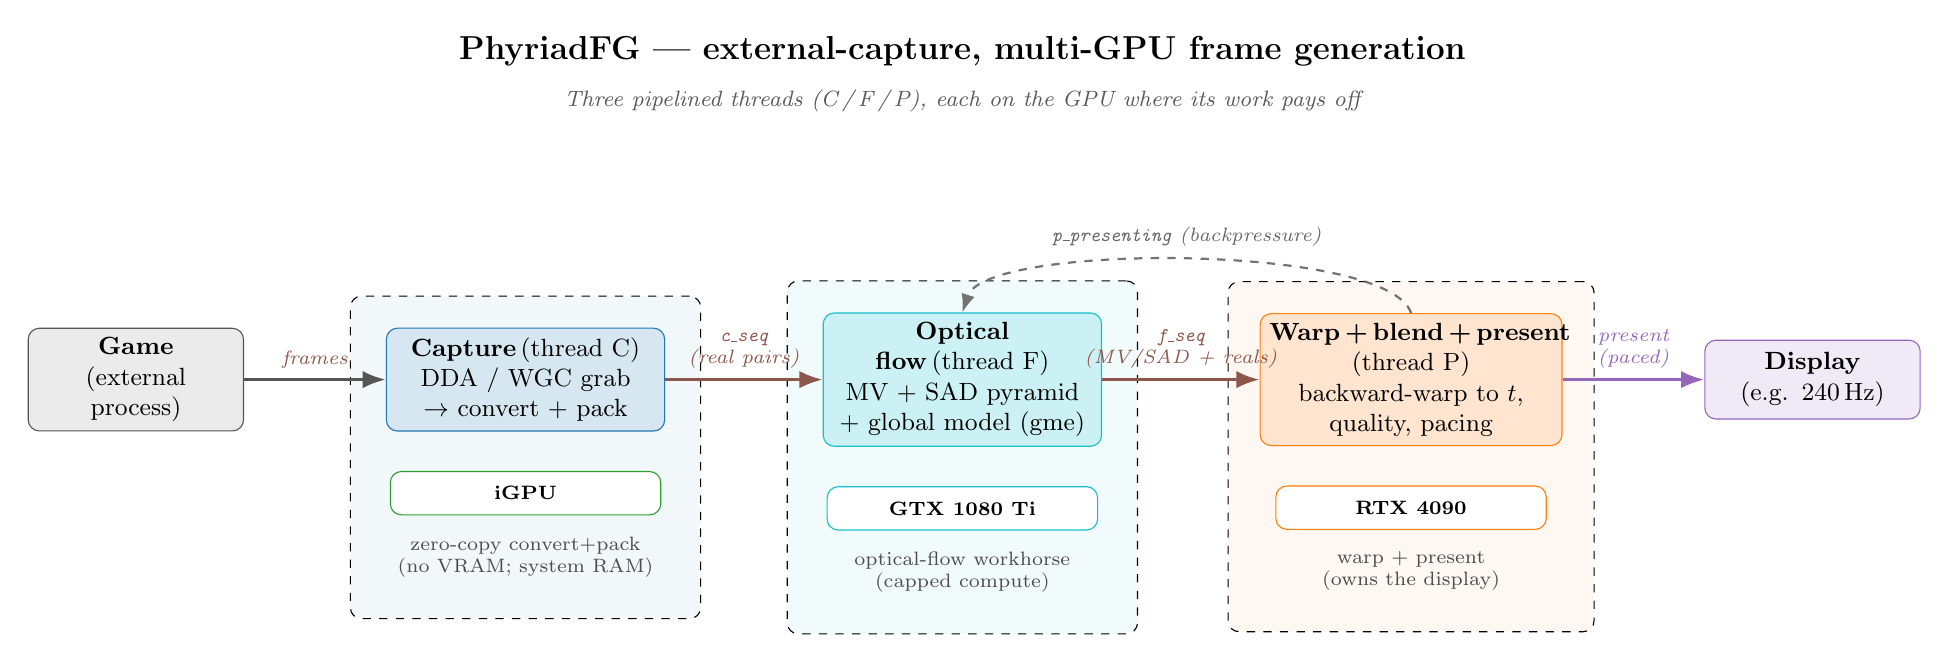
\begin{tikzpicture}[
  font=\sffamily, >=Latex, node distance=10mm,
  ext/.style   ={draw, rounded corners, minimum height=1.0cm, text width=2.5cm, align=center, font=\small, fill=Lgame!12, draw=Lgame},
  work/.style  ={draw, rounded corners, minimum height=1.0cm, text width=3.3cm, align=center, font=\small},
  badge/.style ={draw, rounded corners, minimum height=0.55cm, text width=3.2cm, align=center, font=\scriptsize\bfseries, fill=white},
  lane/.style  ={draw, dashed, rounded corners, inner sep=4mm},
  ringlab/.style={midway, above, font=\scriptsize\itshape, text=Lring, align=center},
  rolelab/.style={font=\scriptsize, text width=3.4cm, align=center, text=black!70},
]

% ── External: the game ───────────────────────────────────────────────
\node[ext] (game) {\textbf{Game}\\(external process)};

% ── Thread C — capture, on the iGPU ──────────────────────────────────
\node[work, fill=Lcapture!18, draw=Lcapture, right=18mm of game] (cap)
  {\textbf{Capture}\,(thread C)\\DDA / WGC grab\\$\to$ convert + pack};
\node[badge, draw=Ligpu, below=5mm of cap] (igpu) {iGPU};
\node[rolelab, below=1.5mm of igpu] (igpurole) {zero-copy convert+pack\\(no VRAM; system RAM)};

% ── Thread F — optical flow, on the 1080 Ti ──────────────────────────
\node[work, fill=Lflow!22, draw=Lflow, right=20mm of cap] (flow)
  {\textbf{Optical flow}\,(thread F)\\MV + SAD pyramid\\+ global model (gme)};
\node[badge, draw=L1080, below=5mm of flow] (g1080) {GTX 1080 Ti};
\node[rolelab, below=1.5mm of g1080] (g1080role) {optical-flow workhorse\\(capped compute)};

% ── Thread P — warp + present, on the 4090 ───────────────────────────
\node[work, fill=Lwarp!20, draw=Lwarp, right=20mm of flow, text width=3.6cm] (pres)
  {\textbf{Warp\,+\,blend\,+\,present}\\(thread P)\\backward-warp to $t$,\\quality, pacing};
\node[badge, draw=L4090, below=5mm of pres] (g4090) {RTX 4090};
\node[rolelab, below=1.5mm of g4090] (g4090role) {warp + present\\(owns the display)};

% ── Display ──────────────────────────────────────────────────────────
\node[ext, right=18mm of pres, fill=Lpresent!14, draw=Lpresent] (disp) {\textbf{Display}\\(e.g. 240\,Hz)};

% ── Data flow (FgContext: SPSC rings + sequence counters) ────────────
\draw[->, very thick, Lgame] (game) -- (cap) node[ringlab]{frames};
\draw[->, very thick, Lring] (cap)  -- (flow) node[ringlab]{\texttt{c\_seq}\\(real pairs)};
\draw[->, very thick, Lring] (flow) -- (pres) node[ringlab]{\texttt{f\_seq}\\(MV/SAD + reals)};
\draw[->, very thick, Lpresent] (pres) -- (disp) node[ringlab, text=Lpresent]{present\\(paced)};

% backpressure P -> F
\draw[->, dashed, thick, black!55] (pres.north) to[out=108,in=72,looseness=0.42]
  node[midway, above=0.5mm, font=\scriptsize\itshape, text=black!60]{\texttt{p\_presenting} (backpressure)} (flow.north);

% ── title strip ──────────────────────────────────────────────────────
\node[font=\large\bfseries, above=30mm of flow, anchor=south] (title)
  {PhyriadFG --- external-capture, multi-GPU frame generation};
\node[font=\footnotesize\itshape, below=0.5mm of title, text=black!65]
  {Three pipelined threads (C\,/\,F\,/\,P), each on the GPU where its work pays off};

% ── group boxes (thread lanes) on the background layer ───────────────
\begin{scope}[on background layer]
  \node[lane, fill=Lcapture!6,  fit=(cap)(igpu)(igpurole)] {};
  \node[lane, fill=Lflow!6,     fit=(flow)(g1080)(g1080role)] {};
  \node[lane, fill=Lwarp!6,     fit=(pres)(g4090)(g4090role)] {};
\end{scope}

\end{tikzpicture}
\end{document}
